\begin{titlepage}
  \thispagestyle{titlepage}
  \begin{center}
  %{\LARGE \myuniversity}\\[5mm]
  \begin{figure*}[h]
   \hbox{}\hfill
   \begin{minipage}[t]{9cm}
			 \centering
			 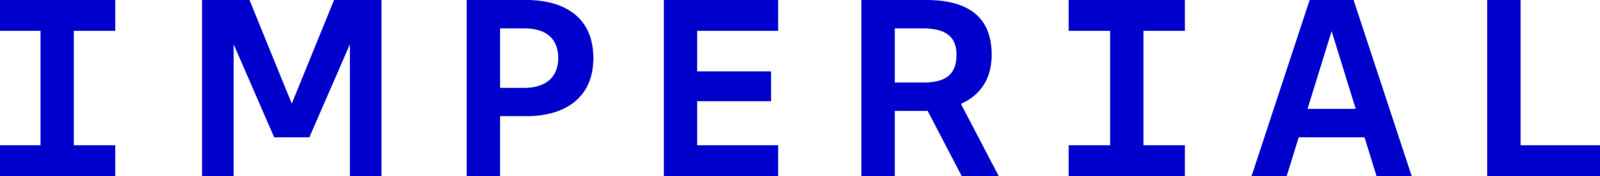
\includegraphics[width=8cm]{logos/Imperial_College_London_new_logo.png}
   \end{minipage}
   \hfill\hbox{}
  \end{figure*}
  {\large \myschool\\ \mydepartment}\\[10mm]
  %{\LARGE \kindOfThesis}\\[10mm]
		%{\large\bf \titleOfThesis}\\[10mm]
		{\Large\bf Physically Informed Machine Learning \\
        for Functional Materials}\\[10mm]
  {\small Author:}\\[1mm]
  {\Large\bf \myfirstname~\mylastname}\\[5mm]
  
  {\small \today}\\[5mm]
  
  \vspace{2cm}
  \renewcommand{\arraystretch}{0.9}
\begin{tabular}{C{0.45\textwidth}}
\small \textbf{Supervisors:} \\[1mm]
\textbf{\large Dr Jarvist Moore Frost} \\[1mm]
\small Department of Chemistry\\
\small Imperial College London  \\
\small 80-92 Wood Lane\\
\small London W12 7TA \\
\end{tabular}
  %\renewcommand{\arraystretch}{.9}
  %\begin{tabular}{cc}
%	{\small  Supervisor:} \\[1mm]
%	{\Large Dr Jarvist Moore Frost} \\[1mm]
  %  {\small Department of Chemistry} \\	
%	{\small \myuni} \\			
%	%{\small \myunistreet} \\
%	%{\small \myunizipcity}\\
  %  {\small 80-92 Wood Lane} \\
%	{\small London W12 7TA}	\\
 % \end{tabular}
  
\vspace{1cm}
{\small Submitted in partial fulfilment of the requirements for the degree of Doctor of Philosophy of Imperial College London}\\[1mm]
\renewcommand{\arraystretch}{1}
  \end{center}
\end{titlepage}

\thispagestyle{empty}
\vspace*{\fill}
\begin{minipage}{.95\textwidth}
\textbf{\mylastname,~\myfirstname:}\\
\emph{\titleOfThesis}\\
\kindOfThesis, \myuni \\
\myplace, \myyear.
\end{minipage}

\cleardoublepage

% =============================================================================

%%%%%%%%%%%%%%%%%%%%%%%%%%%%%%%%%%%%%%%%%%%%%%%%%%%%%%%%%%%%%%%%%%%%%%%%%%%%%
%%% Inhaltsverzeichnis
%%%%%%%%%%%%%%%%%%%%%%%%%%%%%%%%%%%%%%%%%%%%%%%%%%%%%%%%%%%%%%%%%%%%%%%%%%%%%
\newpage
% =============================================================================
\thispagestyle{plain}
\phantomsection
\section*{\Huge Statement of Originality}
%\addcontentsline{toc}{chapter}{Statement of Originality}
%englisch summary of this work
\paragraph{}
\label{SoO}
The thesis titled "Physically Informed Machine Learning for Functional Materials" submitted to Imperial College London for the degree of Doctor of Philosophy is my original work and has not been submitted for any other degree or qualification at any other institution. I, Keerati PK Keeratikarn, hereby declare this assertion.
\paragraph{}
This thesis is the result of my independently conducted research and analysis, and I confirm that all sources and references have been appropriately acknowledged.  I have maintained the academic integrity and ethical standards that Imperial College London expects, and all contributions from other sources have been appropriately acknowledged.
\paragraph{}
I accept that this work may be subject to plagiarism and AI detection software and hereby verify that the content of this thesis is devoid of any form of academic dishonesty.

\newpage
% =============================================================================
\thispagestyle{plain}
\phantomsection
\section*{\Huge Copyright Statement}
%\addcontentsline{toc}{chapter}{Copyright Statement}
%englisch summary of this work
\paragraph{}
\label{CS}
The copyright of this thesis rests with the author. Unless otherwise indicated, its contents
are licensed under a \href{https://creativecommons.org/licenses/by-nc-nd/4.0/}{Creative Commons Attribution-NonCommercial-NoDerivatives 4.0 International Licence} (CC BY-NC-ND 4.0).
\paragraph{}
Under this licence, you may copy and redistribute the material in any medium or format
on the condition that you credit the author, do not use it for commercial purposes and do
not distribute modified versions of the work.
\paragraph{}
When reusing or sharing this work, ensure you make the licence terms clear to others by
naming the licence and linking to the licence text.
\paragraph{}
Please seek permission from the copyright holder for uses of this work that are not included
in this licence or permitted under UK Copyright Law.
\newpage
% =============================================================================
\thispagestyle{plain}
\phantomsection
\section*{\Huge Abstract}
\addcontentsline{toc}{chapter}{Abstract}
%englisch summary of this work
\paragraph{}
\label{abs}
This thesis investigates the incorporation of physically informed machine learning techniques—particularly Gaussian Process (GP) regression \cite{RasmussenW06} and Atomic Cluster Expansion (ACE) \cite{Drautz2019}—to effectively study and model the complex physical behaviours of functional materials \cite{Deringer2021, Musil2021}. Understanding the electronic, thermal, and optoelectronic properties and applications of these materials requires accurate atomistic modelling. The atomistic modelling continues to pose computational difficulties due to the sophisticated anharmonic effects in crystalline inorganic systems and the complex electronic coupling dependencies in organic semiconductors.

The first section presents a derivative Gaussian Process framework \cite{Solak2002,mchutchon_dierentiating_2013, GarijodelRo2019, Kaappa2021, Deringer2021}, (\textsc{GPFC.jl} \cite{https://doi.org/10.48550/arxiv.2405.05113,GitHub}) that effectively evaluates harmonic and cubic anharmonic lattice force constants directly from data obtained through density functional theory (DFT) \cite{Togo2015,Togo2015-qf,Phonopy_toolkit,phonopy}.  This GP-based approach significantly improves computational efficiency, surpassing conventional finite-displacement techniques in predicting phonon dispersion, lifetimes, and thermal conductivity. Our model assesses multiple descriptor strategies, encompassing Cartesian and phonon-based representations, emphasising their influence on accuracy and computational efficiency.

The second section enhances the Atomic Cluster Expansion methodology \cite{Drautz2019} to precisely predict charge transfer integrals essential for charge transport in organic semiconductor materials.  ACE models (\textsc{ACEpotential.jl} \cite{Witt2023}), employing systematically developed symmetry-adapted descriptors \cite{Dusson2022}, effectively capture the electronic coupling's dependence on molecular orientation and separation in various molecular dimers, including naphthalene, thiophene, ethylene, and their fluorinated derivatives.  Our results underscore the significance of descriptor selection and illustrate enhanced model generalisation across chemical systems.

 Our research collectively establishes a unified methodology that integrates rigorous physical insights with sophisticated machine learning techniques.  This integration greatly enhances the computational resources for predicting material properties, facilitating efficient exploration and precise optimisation of innovative functional materials. The thesis concludes by delineating future research avenues, encompassing computational improvements, sophisticated descriptor formulation, and applications to non-equilibrium and real-time dynamic processes.
\newpage
% =============================================================================
\thispagestyle{plain}
\phantomsection
\section*{\Huge Acknowledgements}
%\addcontentsline{toc}{chapter}{Acknowledgements}
%englisch summary of this work
\paragraph{}
I would like to extend my most heartfelt appreciation to all those who have provided me with assistance during my doctoral studies and thesis.
 
Initially, I am profoundly appreciative of my supervisors, Dr. Jarvist Moore Frost.  I am grateful for your unwavering support, encouragement, and invaluable guidance during this research.  Your expert advice and insightful feedback are greatly appreciated.
You have played a critical role in my development as an academic and in my motivation as a scientist.

I am grateful to the Ministry of Education, Thailand, for providing me with a fully funded scholarship that has spanned my entire academic career, the Development and Promotion of Science and Technology Talent project (DPST). 

I am grateful to Prof. Christoph Ortner, Dr. William Chuck Witt, and Cheuk Hin Ho (Jerry) for their unwavering support.  They consistently offer assistance, provide guidance on how to apply their coding program to my research, and provide a comprehensive understanding.

I am grateful to the Imperial Physics and Chemistry Departments for providing the requisite resources and a supportive environment for my research.  In the same vein, I am extremely grateful for the administrative and technical assistance provided by the Matter Group. 

I am unable to express my gratitude to the Frost group members, both past and present, for their unwavering support and encouragement throughout the duration of this PhD.  I am particularly grateful to Bradley Andrew Alan Martin, Hanbo~Yang, Lucius Liu, and Jack Coker for accompanying me on this academic journey, particularly during the COVID-19 pandemic.  I will always cherish the time we have shared, not only for academic-related activities but also for Friday game nights, particularly during the initial phase of my PhD..  You all have been so supportive, helpful, and have made me chuckle so much.  I am grateful to Yande, Ingvars, Ryo, and the new Frost Group cohort for contributing to the second half of my PhD. I always wish for Yande's residence when we shared hotpot. 

I am deeply grateful to my family and friends for their unwavering support, patience, and understanding throughout the difficult periods of this PhD. Their unwavering affection and encouragement provided me with the determination and fortitude to persist. 

I extend thanks to the Southamton community for consistently hosting Thai meal parties, and I also extend my gratitude to the DOTA2 team for providing an unparalleled level of relaxation and enjoyment.

I would like to express my deepest gratitude to my exceptional partner, Jasmine~(Ja).  Over the past four and a half years, I am deeply grateful for your unwavering and sincere love and support. I am unable to do so without your presence.  I have a deep affection for you.

Lastly, I would like to express my gratitude to my mom, Nus, and my dad, Sung.  Every step of the way, you have both been physically and remotely present, consistently believed in me, and consistently provided me with support.  I have a deep affection for both of you.  I am grateful to both of you for your assistance.

\newpage
% =============================================================================
%\renewcommand{\baselinestretch}{2}
\setcounter{tocdepth}{2}
\tableofcontents
\newpage
% =============================================================================
\thispagestyle{plain}
\phantomsection
\addcontentsline{toc}{chapter}{List of Publications}
\section*{\Huge List of Publications}
\begin{itemize}
    \item Keerati Keeratikarn, Jarvist Moore Frost
    \textit{Anharmonic phonons with Gaussian processes},
    arXiv:2405.05113, 2024. (Summitted to IOP Science: Machine Learning: Science and Technology)
    \item Keerati Keeratikarn, Jarvist Moore Frost
    \textit{Machine learning intermolecular transfer integrals with compact atomic cluster representations},\\ 
    arXiv:2511.06551, 2025. (Summitted to Physical Review B)
\end{itemize}
\newpage
% ==============================================

\thispagestyle{plain}
\phantomsection
\addcontentsline{toc}{chapter}{List of Figures}
\listoffigures
\newpage
% =============================================================================
\thispagestyle{plain}
\phantomsection
\addcontentsline{toc}{chapter}{List of Tables}
\listoftables
\newpage
% =============================================================================

% Print the nomenclature list (if you prefer nomencl)
%\printnomenclature
% ----------------------------------------------

% =============================================================================
%% -------------------------------------------------
% Acronym list (compiled with glossaries package)
\thispagestyle{plain}
\phantomsection
\section*{\Huge List of Acronyms}% or \section*
\addcontentsline{toc}{chapter}{List of Acronyms}
% Acronym Table
%-------------------------------------------------
% -------------------------------------------------
% Acronym table (two columns, needs \usepackage{booktabs})
% -------------------------------------------------
\begin{center}
\begin{tabular}{p{2.2cm} p{10.5cm}}
\textbf{\large Acronym} & \textbf{\large Definition / brief description}\\
\midrule\midrule
ACE   & Atomic Cluster Expansion – symmetry-adapted many-body basis\\
ANN   & Artificial Neural Network – nonlinear statistical learning model\\
DFT   & Density Functional Theory – first-principles \\
      & electronic-structure method\\
DIPRO & Dimer Projection method – projects dimer MOs onto \\
      & monomers\\
ESD   & Energy-Splitting-in-Dimer method – estimates transfer integrals from MO splitting\\
FC2   & Second-order (harmonic) force constants\\
FC3   & Third-order (cubic) force constants\\
FDM   & Finite Displacement Method – numerical differentiation for FCs\\
GAP   & Gaussian Approximation Potentials – machine-learned interatomic potentials\\
GP    & Gaussian Process – Bayesian non-parametric regression\\
GPFC  & Gaussian-Process-derived force constants (FC2/FC3)\\
HOMO  & Highest Occupied Molecular Orbital\\
LUMO  & Lowest Unoccupied Molecular Orbital\\
LBTE  & Linearised Boltzmann Transport Equation – phonon transport\\
MBPT  & Many-Body Perturbation Theory – anharmonic phonon interactions\\
\bottomrule
\end{tabular}
\end{center}
\newpage
\begin{center}
\begin{tabular}{p{2.2cm} p{10.5cm}}
\textbf{\large Acronym} & \textbf{\large Definition / brief description}\\
\midrule\midrule
PES   & Potential Energy Surface – multidimensional energy landscape\\
RBF   & Radial Basis Function – kernel in GP and ACE radial transforms\\
RDF   & Radial Distribution Function – histogram of pairwise distances\\
SMRT  & Single-Mode Relaxation-Time approximation – simplified phonon scattering\\
VASP  & Vienna \textit{Ab initio} Simulation Package – plane-wave DFT code\\
\bottomrule
\end{tabular}
\end{center}
\newpage


%% -------------  List of Symbols -------------
\thispagestyle{plain}
\phantomsection
\section*{\Huge List of Symbols}% or \section*
\addcontentsline{toc}{chapter}{List of Symbols}

\begin{center}
\begin{tabular}{p{2.2cm} p{8.5cm} p{2.cm}}
Symbol & Meaning (brief description) & Units \\
\midrule\midrule
$a,\,b$               & Molecular sites (donor / acceptor) & -- \\
$\alpha,\beta,\gamma$ & Cartesian coordinate directions ($x,y,z$) & -- \\
$\kappa$              & Atom index inside a unit cell              & -- \\
$l$                   & Unit-cell index                            & -- \\
$\mathbf{R}^{0}_{l\kappa}$ & Equilibrium position of atom $\kappa$ in cell $l$ & Å \\
$u^{\alpha}_{l\kappa}$ & Displacement of atom $\kappa$ ($\alpha$ component) & Å \\
$\Phi^{(n)}$          & $n$-th order lattice force-constant tensor & eV Å$^{-n}$ \\
$D_{\alpha\beta,\kappa\kappa'}(\mathbf{q})$ & Dynamical matrix element & eV amu$^{-1}$ \\
$\mathbf{q}$          & Phonon wave-vector in the Brillouin zone   & rad Å$^{-1}$ \\
$\omega_{j}(\mathbf{q})$ & Phonon angular frequency (branch $j$) & rad s$^{-1}$ \\
$\epsilon^{\alpha}_{\kappa j}(\mathbf{q})$ & Phonon polarisation vector & -- \\
$n_{j}(\mathbf{q})$   & Bose–Einstein occupation number           & -- \\
$k_{\mathrm B}$       & Boltzmann constant                        & eV K$^{-1}$ \\
$\hbar$               & Reduced Planck constant                   & eV s \\
$C_V$                 & Isochoric heat capacity                   & eV K$^{-1}$ \\
$\tau_{j}(\mathbf{q})$ & Phonon lifetime                           & ps \\
$J_{ab}$              & Electronic transfer integral (coupling) between sites $a,b$ & eV \\
$\varepsilon_{a}$     & Site (diabatic) energy on molecule $a$     & eV \\
$S_{ab}$              & Orbital overlap integral $\langle\psi_a|\psi_b\rangle$ & -- \\
$k$                   & Charge-transfer rate (Marcus theory)       & s$^{-1}$ \\
$\lambda$             & Reorganisation energy                     & eV \\
$\Delta G$            & Gibbs free-energy change                  & eV \\
$T$                   & Finite temperature                      & K \\
\bottomrule
\end{tabular}
\end{center}
\newpage
\begin{center}
\begin{tabular}{p{2.2cm} p{8.5cm} p{2.cm}}
Symbol & Meaning (brief description) & Units \\
\midrule\midrule
$k(\mathbf{x},\mathbf{x}^\ast)$ & Gaussian-process kernel function  & -- \\
$\sigma_{o}$          & GP kernel output scale                    & (var) \\
$\ell$                & GP kernel length scale                    & Å \\
$\mathbf{x}$          & Atomic-environment descriptor (Cartesian) & Å \\
$y(r_{ij})$           & Agnesi radial transform used in ACE        & -- \\
$B_{nlm}$             & ACE basis function of order $(n,l,m)$      & -- \\
\bottomrule
\end{tabular}
\end{center}
\newpage
% Print the nomenclature list (if you prefer nomencl)
%\printnomenclature
% ----------------------------------------------


%\addcontentsline{toc}{chapter}{Algorithmenverzeichnis}
%\listofalgorithms
%\todo{Anleitung Algorithmen schreiben: \url{http://en.wikibooks.org/wiki/LaTeX/Algorithms}}


%are only symmetric (invariant under the permutation of derivative operation. In fact, the GPFCs, however, should satisfy the crystal (translational and rotational) symmetry. To address this symmetry problem, the crystal symmetry need to be included in the derivative GP model to obtain the practical GP model which can be generally applied to a crystal structure.

\newpage
% =============================================================================


%\thispagestyle{plain}
%\phantom{.}
%\vspace{70mm}

%\begin{center}
	%\todo[inline]{This section is optional! It is basically an motivational cite for this work as it can be found in many books. Example is provided}
	%\textit{
		%\vspace{0.5cm}
		% validation of clustering structures is \\
		%the most difficult and frustrating part of cluster analysis. \\ 
		%\vspace{0.5cm}
		%Without a strong effort in this direction, \\
        %cluster analysis will remain a black art 
        %accessible only to those \\
        %true believers who have experience and great courage.}
%\end{center}
%\begin{flushright}
%	\citet{Jain1988}
	%Anil K. Jain and Richard C. Dubes
%\end{flushright}

%\uselengthunit{mm}
%textwidth=\printlength{\textwidth}\\
%textheight=\printlength{\textheight}\\
%top=\printlength{\top}\\

% =============================================================================
% =============================================================================

